\section{Problem Statement}
\label{sec:problemStatement}

In this section, we motivate our work in the context of ensuring the integrity and confidentiality of IO data between the user and the remote servers. We also analyze existing research works that tackle the relevant problem. We explain how these works lack a proper solution and report the observations we derive from them. Lastly, we present the required security properties of \name that we obtain from the observations.

\subsection{Motivation: Secure IO with Remote Safety-critical System}

A user communicates with a remote server through a \emph{host} system that is typically a standard PC (specifically $x86$ architecture), which gives the host access to the raw IO data that is exchanged between the user and the remote server. The host consists of large and complex system software such as the operating system, device drivers, applications such as browser, and a diverse set of hardware components that expose the host to a large attack surface. An adversary that controls the user's host can alter user intentions, i.e., it can perform arbitrary actions on behalf of the user, modify the input parameters, or show wrong information to the user. Such an adversary is very powerful and difficult to be detected or prevented by a remote server. Hence, existing defense standards for web UI are ineffective as the browser is untrusted also. The consequences of such attacks might be severe when applications that control remote safety-critical systems are targeted. The attacker can pass the wrong input to a remote safety-critical system such as a medical device, power plant, etc., or leak sensitive information such as credentials for e-banking, candidate preference in the e-voting, etc.



%In this paper, we primarily target the trusted path problem to a remote server (such as a remote PLC, web server or remotely accessible medical device, etc.) that is being accessed from a browser running on a commodity $x86$ host.


\subsection{Analysis of Existing and Strawman Solutions}
\label{sec:problemStatement:existingSolution}

There are two broad categories of existing solutions that address the problem of trusted paths for IO devices in the presence of a compromised host as illustrated in Figure~\ref{fig:relatedWorksTree}: \textbf{A.}~Solutions where unprotected user interaction first happens and then a trusted component (transaction confirmation device) is used to ensure input integrity,
and \textbf{B.}~Solutions where a trusted component captures the user's input/output and then securely mediates them to the destination. The trusted component can be a hypervisor, or an external hardware, etc. %Table~\ref{tab:relatedWorks} provides a comprehensive analysis is trusted path literature.

\myparagraph{A.~Transaction confirmation devices} In their paper, Filyanov et. al~\cite{filyanov2011uni} proposed transaction confirmation device that requires the user to use a separate device to confirm the input parameters. Systems such as ZTIC~\cite{weigold2011secure} use an external device with display and smartcard attachment to ensure the integrity of the user inputs. Android OS also provides a similar mechanism to confirm protected transactions~\cite{android_confirm}. 
However, these approaches suffer from three significant drawbacks: i) the risk of \emph{user habituation} -- users confirming transactions without looking to the actual data~\cite{anderson2016warning},
ii) \emph{usability} -- interacting with a small device can be cumbersome, and iii) only \emph{simple UI} can be supported -- transaction confirmation is not suitable for complex interaction, rather than simple text-based inputs.


\begin{figure}[t]
\scriptsize
    \centering
    \begin{tikzpicture}[
solved/.style={rectangle,draw,fill=purple!40, rounded corners, align=center},
not/.style={rectangle, fill=white, align=center},
neutral/.style={rectangle, draw, rounded corners, align=center, fill=black!5}
]]
  \node[not](empty) {};
    \node[neutral, right=3cm of empty](root) {Trusted path}
    child { node[neutral, yshift=10pt, xshift=-70pt, yshift=10pt] (tc) {\textbf{A.} Transaction\\ confirmation Device}}  
    child { node[neutral, yshift=10pt, xshift=10pt, yshift=15pt] (td) {\textbf{B.} Trusted intermediary}       
        %child { node[neutral, yshift=0pt, xshift=-30pt, yshift=7pt] (tee) {\textbf{B2.} TEE}}
      %child { node[neutral, yshift=2pt, xshift=-50pt, yshift=7pt] (br) {\textbf{B1.} Browser-based}}   
     child { node[neutral, yshift=9pt, xshift=-25pt] (hv) {\textbf{B1.} Hypervisor-based}} 
     child { node[neutral, yshift=9pt, xshift=0pt] (hw) {\textbf{B2.} External HW}}
    } ; 
      

    \node[below=0cm of hw](gurdion) {\textbf{\name}};
    %\node[below=0cm of tee] {VButton~\cite{li2018vbutton}};
    \node[below=0cm of tc] {Uni-dir~\cite{filyanov2011uni}};
    \node[below=0cm of hv](os) {Overshadow~\cite{Overshadow}};
    \node[below=0cm of os] {SGXIO~\cite{weiser2017sgxio}};
    \node[below=0cm of gurdion] {Fidelius~\cite{Fidelius}};
     %\node[below=0cm of br](ic) {InContext~\cite{blake1998authenticated}};
     %\node[below=0cm of ic] {W3C UI security policy~\cite{w3c_spec}};

    
    \end{tikzpicture}
    
   \caption{\textbf{Existing trusted path solutions} by their approach.}
   \spacesave
     \label{fig:relatedWorksTree}
\end{figure}


\myparagraph{B1.~Trusted hypervisor-based solutions} Trusted hypervisors and secure micro-kernels are also alternatives to achieve Trusted path. Zhou et al.~\cite{zhou2012building} proposed a generic trusted path on $x86$ systems in pure hypervisor-based design. SGXIO~\cite{weiser2017sgxio} combines a TEE and a hypervisor to mitigate the shortcomings of TEEs like SGX (OS controls the IO operations). Nevertheless, solutions based on hypervisors require a large TCB. Formally verified hypervisors offer limited functionalities, therefore making them impractical for average users. One can also argue that a hypervisor that provides a rich set of functionalities has a code size comparable to an actual OS. Also, systems employing TEEs such as Intel SGX open up new attack surfaces that can be exploited by microarchitectural attacks~\cite{van2018foreshadow}.


\myparagraph{B2. External hardware-based solutions} Several existing works propose a trusted path that utilizes an external trusted device. IntegriKey~\cite{IntegriKey} uses a trusted external device that contains a small program which signs all user inputs and sends the signed input to the remote server. The device works as a second factor for input integrity as the remote server verifies if the signed input matches with the input that is sent by the browser running on the untrusted host. However, as the external device is completely oblivious to the display information that the untrusted host renders, not only IntegriKey but also similar systems that do not consider output integrity are vulnerable to UI manipulation attacks. For example, assume that the user's intended input to a textbox is $100$. She types the correct value, but the host maliciously renders $10$ on the screen by not showing the last zero. Thinking that she might have mistyped, the user types another $0$ that makes the recorded input from the user $1000$. This attack violates input integrity as the host can now submit $1000$ to the remote server as a valid input, although it does not represent the user's intention. 
%In Appendix~\ref{appendix:security:protocol}, we provide a formal security proof that shows why systems like IntegriKey or transaction confirmation device that do not provide output integrity also lack input integrity.
%and, the external trusted device also signs $1000$ as the correct input received from the user.

\noindent\emph{$\rightarrow$ Observation 1:} The lack of output integrity -- \emph{the render of user inputs on the screen} -- compromises input integrity.

\begin{figure}[t]
\centering
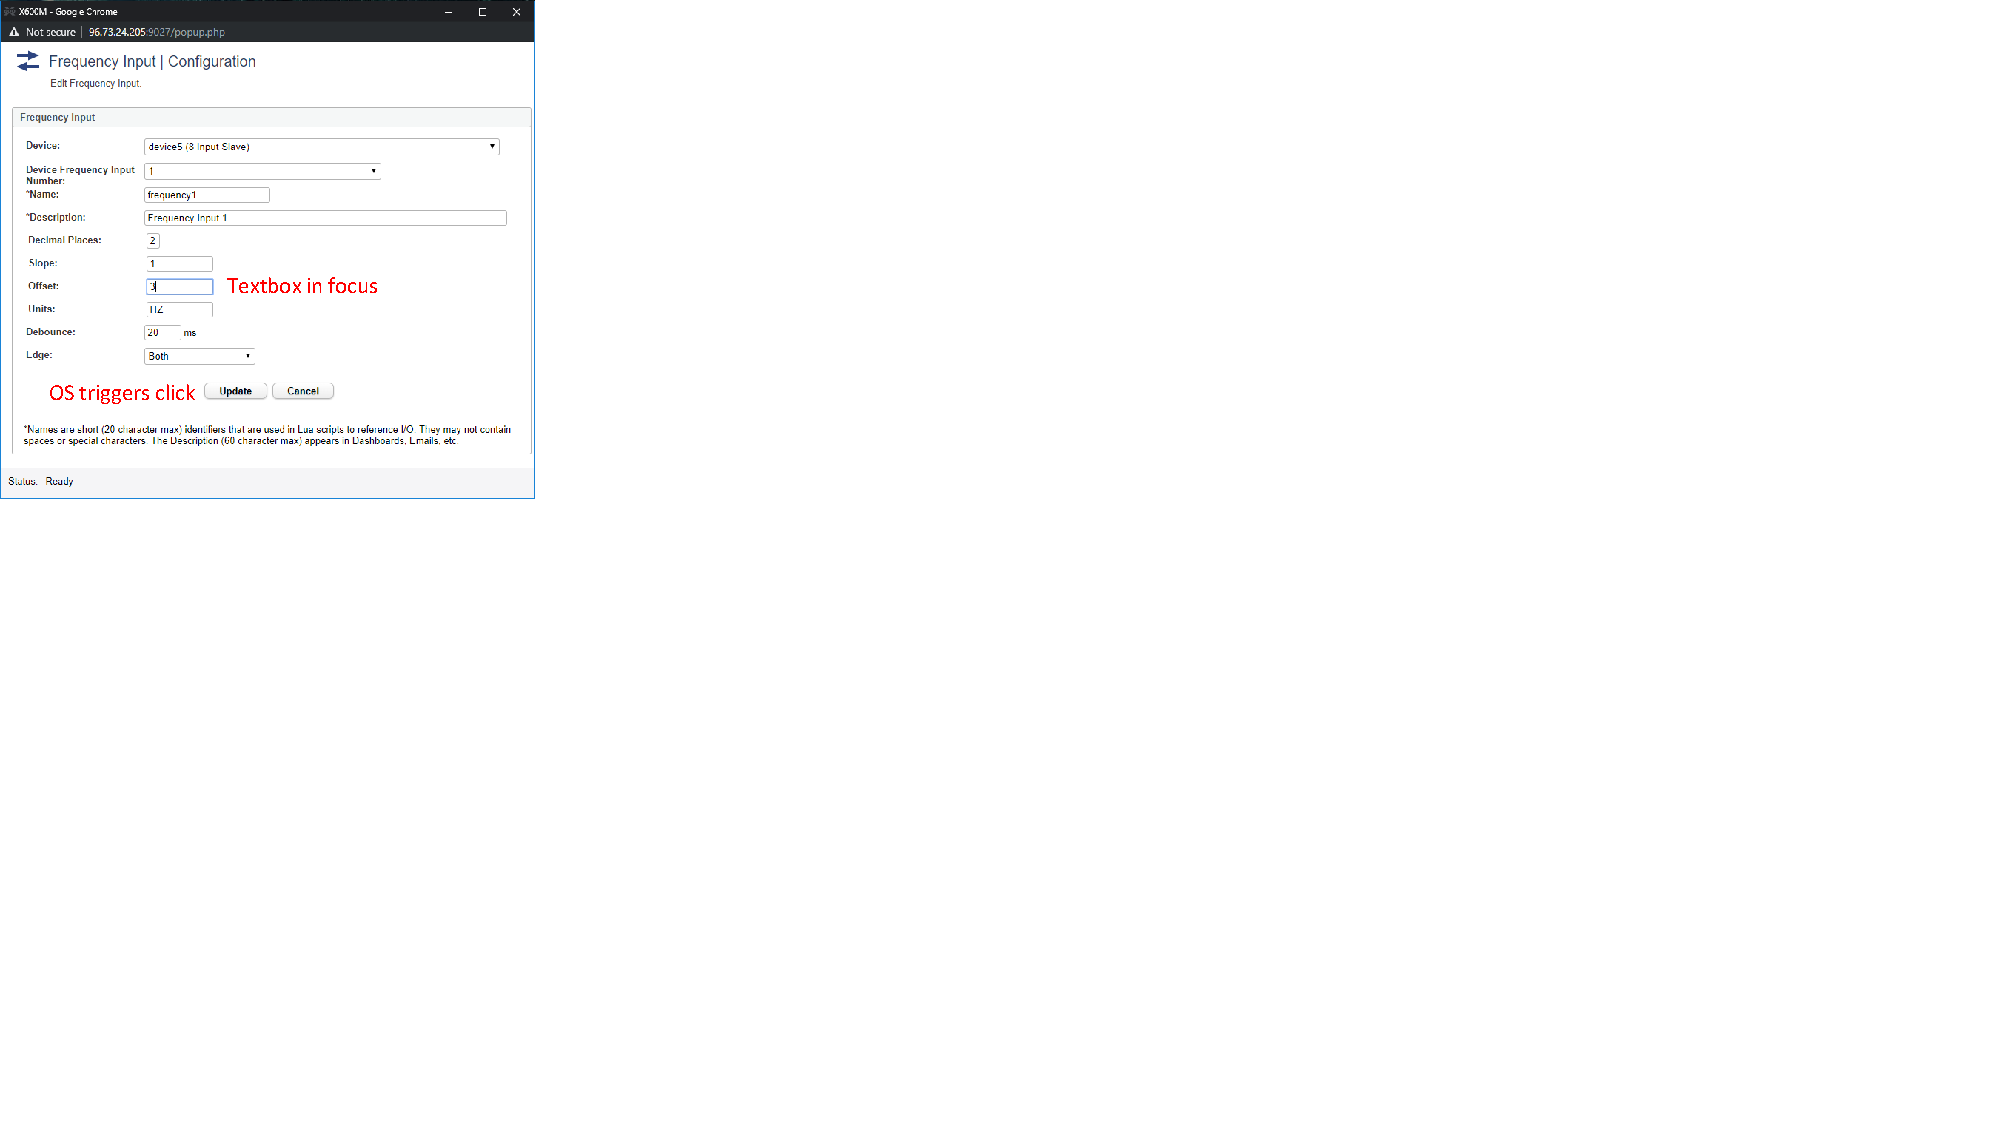
\includegraphics[trim={0 11.5cm 21.8cm 0}, clip, width=0.8\linewidth]{earlyFormSubmission.pdf}
\caption{\textbf{Early form submission attack} is possible on Fidelius~\cite{Fidelius}. The user selects and edits the field \texttt{Units} while the OS triggers \texttt{add} button, causing misconfiguration of a remote safety-critical PLC (Control by Web X-600M~\cite{controlbyweb}).}
\spacesave
\label{fig:clickJack}
\centering 
\end{figure}

Fidelius~\cite{Fidelius} addresses the problem with output integrity by rendering overlays using an external trusted device. Fidelius uses the trusted external device and Intel SGX to create a secure channel between the user IO devices and a remote server. The device intercepts user keystrokes and does not deliver any event to the untrusted host when the user types to secured text fields. Additionally, Fidelius renders an overlay with the user inputs on the screen, which is inaccessible by the host. This way, the untrusted host does not have access to raw inputs while the user sees them rendered on the screen as usual.
%provides secure input and display for the character-based device - keyboard. It uses overlays on the text fields to hide the keyboard input from the compromised host so that the input is only visible to the user. 
A small, trusted bar on display is also overlaid by the device that shows the remote server's identity and the text field that is currently selected. 
However, we observe a number of security and functional issues in Fidelius that we explain in the following.

The overlay contains only the render of the user inputs into text fields, but the rest of the screen is rendered by the untrusted host.
This allows an attacker to modify the instructions on the UI, such as changing the unit of the input (typically described in the label of a text field) that could result in an incorrect input. This problem could be mitigated if the trusted bar includes the legitimate labels of the text fields also, although it would significantly increase the cognitive load to users.

%Fidelius solely relies on the static overlay bar and the LEDs on the external device to ensure the integrity and confidentiality of the input. 
Fidelius already introduces a high cognitive load to users as they need to monitor multiple security indicators simultaneously before filling up one text field. Previous research works~\cite{egelman2008you,sobey2008exploring, anderson2016warning} have shown that systems that require users to observe multiple security indicators %that require the users to observe multiple markers on the screen (and also on an external device) 
do not guarantee security in practice.
Also, in specific scenarios, even the training to properly explain these indicators to users could be a significant drawback for a real deployment.
%as the users require training to familiarize with the system (such as different security indicators).
%Fidelius overlays only user inputs on the screen and keeps them isolated from the host. 

\noindent\emph{$\rightarrow$ Observation 2}: If the \emph{protected output} is provided out-of-context, users are more likely not to verify it. Therefore input integrity can be violated.


Fidelius does not consider the integrity of the mouse pointer and its interaction with UI elements which broadens the attack surface. The lack of mouse support may appear to be a functional limitation, but it has non trivial security issues.
The OS can arbitrarily trigger a mouse click on the submit button of a form while the user is typing and therefore send incomplete data to the server - early form submission attack.
This attack could cause the misconfiguration of a remote system, as illustrated in Figure~\ref{fig:clickJack}. Early form submission may appear to be similar to clickJacking attack, but the fundamental difference between them is that in clickjacking the browser and OS are considered to be trusted. An untrusted OS can simply issue mouse clicks.

Moreover, Fidelius is also vulnerable to clickjacking attacks where the attacker can spawn a fake mouse pointer and trick the user into following it while the real mouse pointer is on a sensitive text field protected by the system. This allows the attacker to fool the user into providing (possibly incorrect) input, while the user thinks that she is interacting with a non-sensitive text field. To prevent such attacks, the user has to look at the security indicators continuously even when she is not doing any security-sensitive task, which is a very strong assumption. 
Thus, not supporting the mouse causes the integrity violation of the keyboard input also.

\noindent\emph{$\rightarrow$ Observation 3:} If not \emph{all the modalities of inputs} are secured simultaneously, none of them can be fully secured.


Finally, the design of Fidelius~\cite{Fidelius} is strictly limited to text-based fields only. As Fidelius does not provide output integrity of the forms, it cannot provide confidentiality to other UI elements such as radio buttons, drop-down menus, sliders, etc.
Microarchitectural attacks on Intel SGX increase significantly the attack surface of the system also~\cite{van2018foreshadow}.


\myparagraph{Strawman solution: Capturing screenshot} This strawman solution uses a trusted device that takes a screenshot when the user executes an action, e.g., mouse click to submit a form. The device then signs the snapshot and transmits it to the server along with the signed input. The remote server verifies the signature and then uses image/text analysis to extract the information from the UI elements such as labels on buttons or markers of a slider, etc. Therefore, the server would detect if the host has manipulated UI elements when presented to the user.

This method is vulnerable to attacks because it does not capture the spatiotemporal user context. This implies that the attacker may show some spacial information on the screen to influence the user that may not be captured by the snapshot. Furthermore, taking a full-screen snapshot could also reveal private information of the user from other applications. Similarly, taking a snapshot does not guarantee that a specific UI has been presented on the screen as the attacker may render the legitimate UI shortly before the device captures the snapshot.
One way to mitigate this problem is to capture a video of user interaction. But such a method requires the host to send large amounts of data to the server, while the server should support video processing for different browsers which is both time and CPU intensive. Lastly, adversarial machine learning techniques~\cite{eykholt2017robust,sitawarin2018rogue} make the image/text recognition techniques insecure against advanced adversaries.


\subsection{Requirements of Security and Functional Properties}
\label{sec:problemStatement:goals}

The lack of security properties and features in the existing solutions provides the necessary security and functional requirements for a trusted path that provides IO integrity and confidentiality and is usable. We can now summarize the observations that we derived from the literature and the strawman solution (refer to Section~\ref{sec:problemStatement:existingSolution}) as following:

\myparagraph{R1. Inter-dependency between input and output} 
The first and second observations from the existing solutions show that the output and input security depend on each other, and they should be considered together. Otherwise, the attacker can manipulate the output to influence the user input.
%The main lesson that we learn from the previous papers is that input and output integrity, and confidentiality cannot be considered in isolation. Rather, they are needed to be secured simultaneously as the output, and the input both influence each other.  

\myparagraph{R2. Inter-dependency between all input modalities} 
Existing web interfaces allow users to complete forms by using different modalities for the user input, namely the keyboard, the mouse, and the touchpad. The third observation shows that a secure system should protect simultaneously all user input modalities to achieve input integrity (against early-form submission and clickjacking).

%If there exist multiple input sources (typically keyboard and mouse), all of them should be protected simultaneously as these input sources influence each other. For example, in a web application scenario, protecting the integrity of only the keyboard input does not provide input integrity as an attacker-controlled host can always execute an early form submission attack.

\myparagraph{R3a. No cognitive load for IO integrity} 
A system that protects IO operations should introduce minimal or no cognitive load to its users for input integrity.
The system should guarantee the output integrity of the legitimate information necessary to complete a form and avoid asking the user to interact with an external device or monitor security indicators out-of-context.

%Output integrity protection can eliminate the actions that lead to high cognitive loads to the user.  Such as using an external device to confirm every transaction, looking to a passive security indicator and confirming actions, etc. The systems that rely heavily on such security measures suffer from input errors that originate from user habituation. Moreover, such designs require user training that makes the system hard to deployment and costly.

\myparagraph{R3b. User attention for IO confidentiality} Preserving the confidentiality of user inputs against a compromised host is a challenging task because the host can simply fool the user to reveal her inputs when the system is not active. Therefore, requiring users to perform a small action, e.g., press a key, before entering confidential inputs is a valid trade-off between usability and security.

%Confidentiality requires active triggering from the user to distinguish the secure part of the screen from ensuring part of the screen if the part of the output provides integrity/confidentiality protection.

\myparagraph{R4. Small trust assumptions and deployability} 
Our goal is to provide the aforementioned rich set of IO and security features with minimal trust assumptions that do not rely on a trusted OS, specialized hypervisor, or TEEs such as Intel SGX. Preferably, the solution should be easy to set up for users, i.e., plug-and-play, and integrate well with the existing infrastructure.  
